\section{Použité algorimy a datové struktury}

\subsection{Tabulka symbolů}

\begin{figure}[htbp]
    \centering
    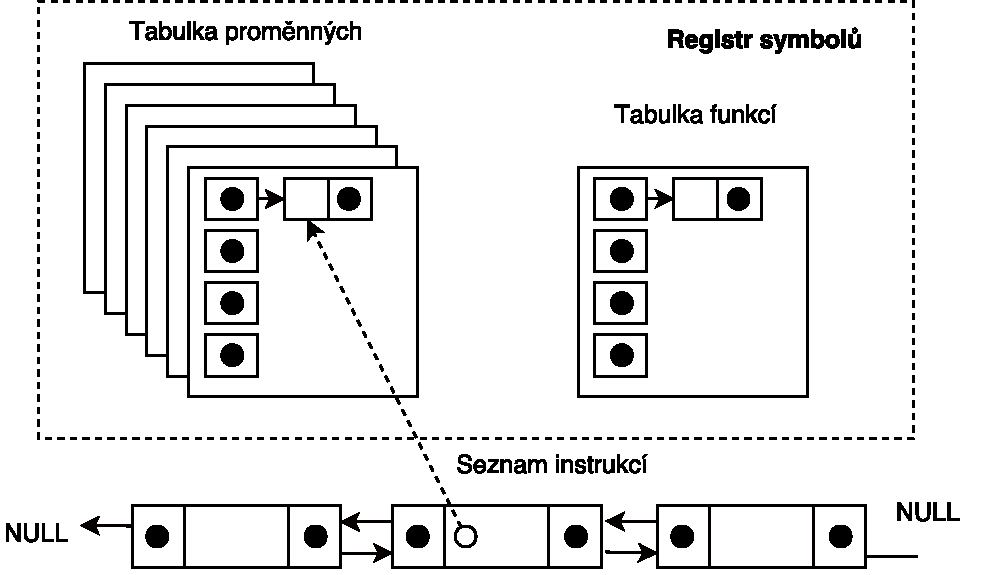
\includegraphics[width=0.6\textwidth, angle=0]{src/assets/symbol_table.pdf}
\end{figure}

Pro implementaci tabulky symbolů jsme zvolili tabulku s~rozptýlenými položkami s~použitým lineárním seznamem pro synonyma.
Tuto strukturu jsme kromě tabulek symbolů funkcí a proměnných použili ke sběru dat v~optimalizátoru cílového kódu. Bylo tedy nutné tuto strukturu implementovat vhodně tak, aby pro každé použití mohla držet různá data ve svých položkách. Existuje tedy základní verze položky \ic!SymbolTableBaseItem!, která zapouzdřuje pouze klíč a ukazatel na další položku v~lineárně svázaném seznamu synonym.

Pro konkrétní použití jsou poté vytvořeny struktury \ic|SymbolVariable| a \ic|SymbolFunction| obsahující nutná data pro tyto symboly (datový typ, rámec, úroveň zanoření resp. návratový typ, seznam parametrů) - tyto struktury obsahují obecnou \ic!SymbolTableBaseItem! vždy na prvním místě, aby bylo možné použít přetypovávání pro algoritmy. Veškeré základní operace nad tabulkou poté fungují nad \ic!SymbolTableBaseItem! pro obecnost algoritmů. Samotná tabulka také může obsahovat ukazatel na funkci, která samotnou položku inicializuje po vytvoření, resp. uvolní před smazáním.

Pro sémantické kontroly v~modulu \ic|ParserSemantic| existuje struktura \ic|SymbolRegister| zapouzdřující tabulku funkcí a zásobník tabulek proměnných. Dále obsahuje čítač pro generování unikátních identifikátorů pro symboly v~cílovém kódu. Zásobník je implementován jako jednosměrně svázaný seznam tabulek proměnných a tabulky jsou do něj vkládány/vyjímány při každé zanoření bloků jazyka IFJ17.

\subsection{Správa paměti}
Pro kontroly neuvolněných paměťových bloků dynamické správy paměti byl vytvořen modul \ic|MemoryManager|, na který je napojen pár maker \ic|memory_alloc| a \ic|memory_free|. Tato makra mají identické rozhraní s~vestavěnými funkcemi \ic|malloc| a \ic|free|, avšak zachovávají informace o~alokovaných \uv{stránkách} paměti, které se vždy uvolňují až na konci běhu programu. Stránky jsou dvousměrně svázány do seznamu pro přístup (\uv{uvoľňování}) s~časovou složitostí $\mathcal{O}(1)$.

\subsection{Optimalizace}
Z~vyšších datových struktur je zde použit \textbf{orientovaný graf a množina}. Z~těch nižších poté obecný dvousměrně svázaný seznam, zásobník implementovaný pomocí jednosměrně svázaného seznamu a tabulka s~rozptýlenými položkami. Množina je zde implementována jako dvousměrně svázaný seznam (\emph{narozdíl od doporučované varianty s~binárním stromem}) vzhledem k~očekávanému nízkému počtu položek v~ní a tím i příznivé časové složitosti $\mathcal{O}(n\cdot log(n))$. Orientovaný graf je implementován jako \textbf{jednorozměrné pole uzlů tohoto grafu} - každý uzel poté obsahuje množinu vstupních a výstupních hran pro konkrétní uzel. V~tomto grafu jsou silně propojené komponenty vyhledávány pomocí \textbf{Tarjanova algoritmu} \footnote{https://en.wikipedia.org/wiki/Tarjan\'s\_strongly\_connected\_components\_algorithm} pro vyhledávání s~časovou složitostí $\mathcal{O}(n)$.